\begin{figure}[p]
\centering
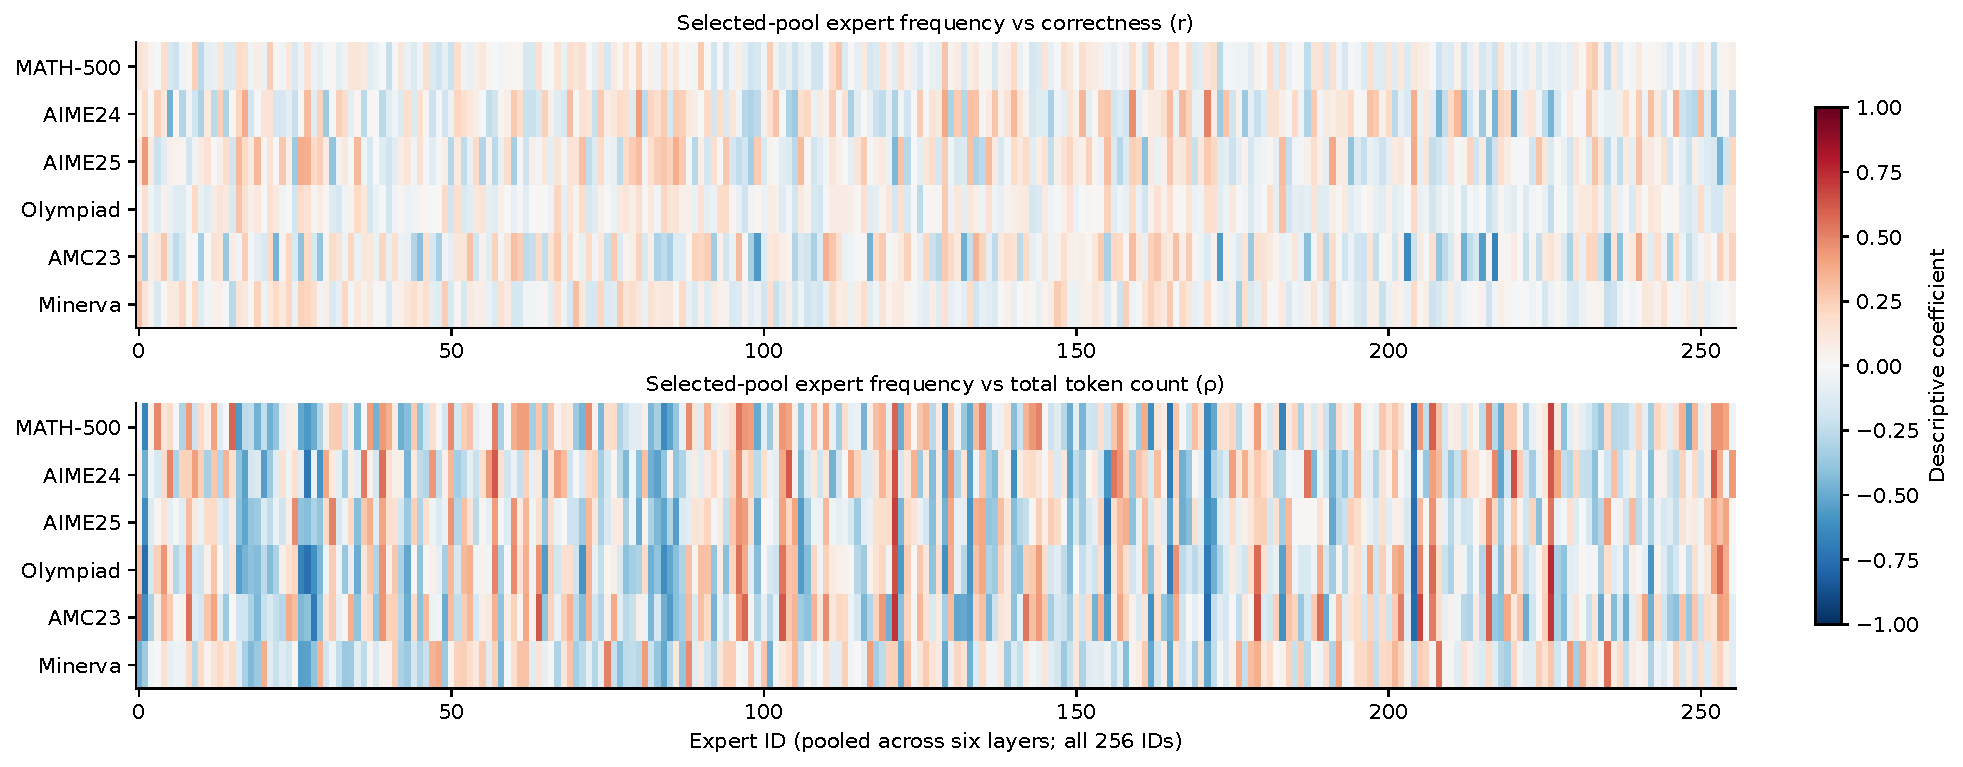
\includegraphics[width=\linewidth]{figures/qwen_expert_outcomes.pdf}
\caption{Selected-pool membership frequency for every expert ID versus
correctness ($r$, top) and total continuation tokens ($\rho$, bottom).
All 256 IDs are shown in their original order for each benchmark. Rates
pool tokens and six layers; the same ID refers to distinct layer-local
modules. These associations do not establish that activating an expert
will improve accuracy or reduce length.}
\label{fig:expert-outcomes}
\Description{Router features are compared with whole-attempt outcomes across six benchmarks; the caption defines the estimates and uncertainty.}
\end{figure}

\paragraph{Metric values associated with accuracy.}
Correlation signs alone do not specify the observed metric ranges associated
with higher accuracy (42:06--45:17). Figure~\ref{fig:router-value-accuracy}
therefore reports accuracy directly against router confidence, the
selection-boundary margin, and the selected/rest mean probability gap.
Bins are computed separately per benchmark; this is an exploratory
whole-continuation analysis, not an online threshold-selection experiment.

\begin{figure}[p]
\centering
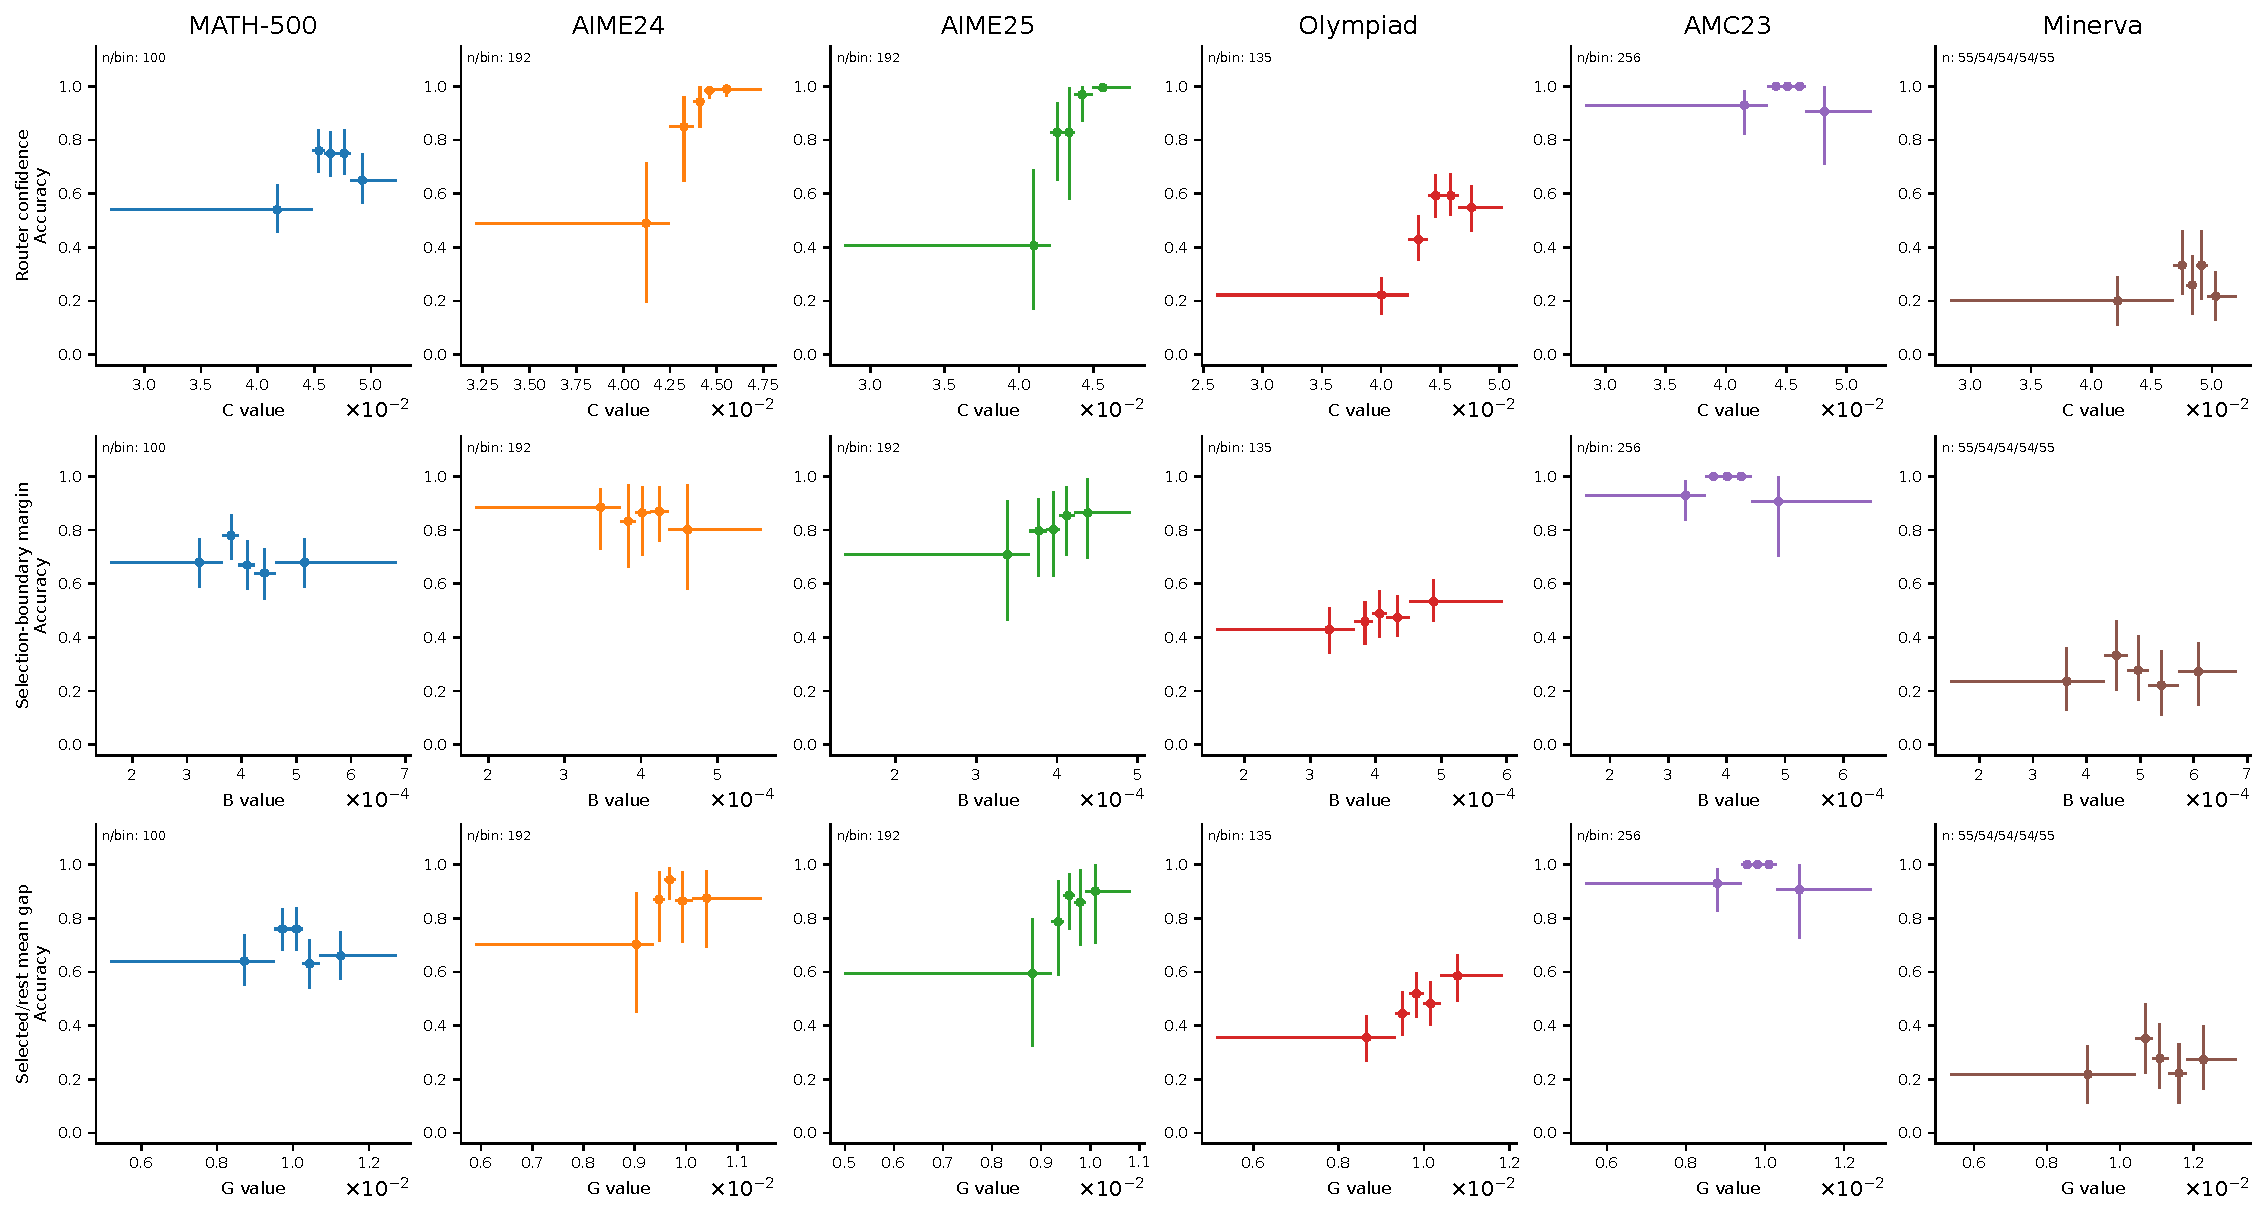
\includegraphics[width=\linewidth]{figures/qwen_router_value_accuracy.pdf}
\caption{Accuracy at observed router-metric values. Each benchmark uses
up to five quantile bins; horizontal bars show actual value ranges, points
show mean values and accuracy, and panel labels give attempt counts
per bin (left to right, or a shared count when equal). Vertical
bars are pointwise 95\% percentile intervals from 500 whole-source-problem
bootstrap resamples within each fixed bin (seed 42). Degenerate intervals
can occur in all-correct/all-incorrect bins and do not imply certainty.
All attempts and limit hits are retained. Bins can share source problems,
so their estimates are not independent; neither bin selection nor length
and termination confounding is addressed by these intervals.}
\label{fig:router-value-accuracy}
\Description{Router features are compared with whole-attempt outcomes across six benchmarks; the caption defines the estimates and uncertainty.}
\end{figure}

\paragraph{Common router notation and unavailable extensions.}
Let $p_{(j)}$ denote the $j$th largest router probability, $E$ the number
of experts, and $k$ the selected count ($E=256$, $k=8$ here). Router
confidence is $C=1-H(p)/\log E$; leading-expert margin is
$M=p_{(1)}-p_{(2)}$; selected probability mass is
$S=\sum_{j\leq k}p_{(j)}$; selection-boundary margin is
$B=p_{(k)}-p_{(k+1)}$; and selected/rest mean gap is
$G=S/k-(1-S)/(E-k)$. Thus $M$ is not a selected-versus-rest statistic.
These model-independent names replace ambiguous top-8/top-9 plot labels
without changing the saved metric definitions.

The requested rank-prefix curves (top 2, 4, 6, then all selected versus
the rest; 20:11--21:07 and 37:29--39:20) require additional probability
summaries. Only the all-selected endpoint $G$ is saved. Separate entropy
of the selected and unselected distributions also cannot be recovered
from global entropy, selected mass, or expert IDs. These extensions
require new feature extraction/replay; no missing curves are fabricated.
